% This must be in the first 5 lines to tell arXiv to use pdfLaTeX, which is strongly recommended.
\pdfoutput=1
% In particular, the hyperref package requires pdfLaTeX in order to break URLs across lines.

\documentclass[11pt]{article}

% Style and Formatting for Camera-Ready PDF
\usepackage{naacl2021}

\usepackage{dblfloatfix}


% Standard package includes
\usepackage{times}
\usepackage{latexsym}

% own packages
\usepackage{tikz}
\usepackage{graphicx}
\usepackage{subcaption}

% For proper rendering and hyphenation of words containing Latin characters (including in bib files)
\usepackage[T1]{fontenc}
% For Vietnamese characters
% \usepackage[T5]{fontenc}
% See https://www.latex-project.org/help/documentation/encguide.pdf for other character sets

% This assumes your files are encoded as UTF8
\usepackage[utf8]{inputenc}

% This is not strictly necessary, and may be commented out,
% but it will improve the layout of the manuscript,
% and will typically save some space.
\usepackage{microtype}

% If the title and author information does not fit in the area allocated, uncomment the following
%
%\setlength\titlebox{<dim>}
%
% and set <dim> to something 5cm or larger.

\title{Deepfakes: The Road towards a General Detection Method}

% Author information can be set in various styles:
% For several authors from the same institution:
\author{Emre Kavak \and Ana Răduțoiu \and Emanuel Rămneanțu \\
        Technische Universität München \\
        \texttt{ \{emre.kavak, ana.radutoiu, emanuel.ramneantu\}@tum.de }}


\begin{document}
\maketitle
\begin{abstract}
Deepfakes (DF) are images and videos where the face of a person is replaced by one of another individual and are usually generated using a machine learning (ML) model. Since deepfakes became a really popular topic in the scientific community, numerous DF generation and detection methods have arisen, thus leading to an increased number of fake content that is present online. Unfortunately, it is not unusual to spot deepfake content created without consent and it often happens that this technology is used in a harmful and hateful ways. Considering this, we can conclude that there is a need for robust deepfake detection methods that can easily identify the faked content. However, most of the state-of-the-art classifiers are only able to recognize deepfakes generated using the same method that was used for testing. In other words, most detectors are not able to generalize to yet unseen DF generation methods. In this work, we analyze this behavior and try to find the reason and a solution for this. 
\end{abstract}

\section{Introduction}
%% Deepfake definition%%
Deepfakes can be described as fake media content where the face of an individual is replaced by another of a different person and are usually created using generative machine learning models. Responsible for this nomenclature is a Reddit user that created a thread called 'r'/deepfakes' \cite{DF_vice} where he would post fake porn videos that used the technology.  Although this method does not inherently have a malicious nature, the debut of deepfakes already shows that they can be used with destructive intentions. State-of-the-art artificial intelligence techniques can yield fake content that often could even trick the human eye and therefore deepfakes represent a threat to personal security. They could be used as a tool for manipulation, humiliation and harm towards the subjects who's faces have been forged and towards the individuals that are watching the deceiving content.  \\

%%Introducing deepfake detection%%
Considering this, the need of robust deepfake detection methods arises as a tool of granting the authenticity of the identities of individuals presented in pictures or videos. In the last years there have been many attempts at generating deepfakes, using different approaches, but also at creating the best detection method which could yield the highest real vs. fake classification accuracy. 

\subsection*{Generating deepfakes}
\begin{figure}
  \centering
    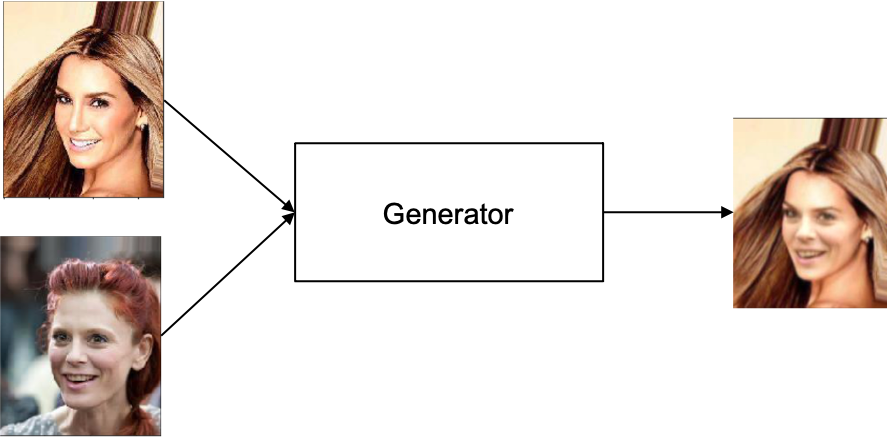
\includegraphics[width=0.4\textwidth]{figures/DFGenerationEx.png}
  \caption{Illustrative, simplifying example of a general generation pipeline \cite{liu2015faceattributes}.}
  \label{fig:dfgeneration}
\end{figure}
Most of the deepfakes are generated using  encoder-decoder pairs (e.g. Autoencoders (AE) or Variational Autoencoders (VAE)) \cite{nguyen2021deep}. For this, two datasets are needed, one of face images of the source subject and one of face images of the target subject, as well as two networks, each trained on one of the datasets. To create the deepfakes, the encoder trained on images of the source subject is coupled with the decoder of the network trained on images of the target. The resulting network will place the face of the source person on the head of the target person, as depicted in figure \ref{fig:dfgeneration}. Other methods use variations of Generative Adversarial Networks (GAN). However, these techniques are usually not used to swap faces, but rather to create brand new ones \cite{karras2020analyzing}. Another category of methods that are used for generating deepfakes use computer vision approaches like facial key point detection, blending and warping and color adjustment \cite{li2020face}. Challenges for deepfake generation methods are creating high quality reenactment images without visible artifacts. This is especially hard to obtain since the image subjects can have different head positions, different skin tones, closed eyes etc. 

\subsection*{Detecting Deepfakes}
For detection, there are mostly two different approaches that can be used. First one is based on identifying specific artifacts that may appear, for example, blending artifacts and double eyebrows. Usually, this is modelled explicitly and the classification algorithm needs hand-crafted features as inputs. The other detection procedure is a more general one that treats the task as a black box binary classification. For this, classifiers are trained on raw images directly, by using a CNN architecture, or features automatically extracted from those images, in which case a shallow classifier might be used. \\
%%Challenges for detection methods == generalization%%
Since most detection methods are data driven, they overfit the dataset that they have been trained on and only learn the specific artifacts of the generation method that was used for creating the deepfakes in the training set. Thus, when the trained models face image samples generated with an unseen generation method, they tend to perform badly and thus indicate that they have no \emph{generalization} power across different generation methods.

\\
Considering this, we can argue the importance of creating a detection method that can generalize to all deepfake datasets, regardless of the training set. This is especially relevant if we are faced with the task of classifying an image or a video that is suspected to be deepfake, but comes from an unknown source. However, it is not trivial to tackle this problem.

In this work, we want to get closer to the goal of finding a detection method with generalization ability. Our \textbf{contributions} for reaching this objective are:
\begin{itemize}
    \item We summarize different deepfake generation methods and create a deepfake database which also includes self-created datasets
    \item We evaluate different detection methods and bring our own modifications to already-existing detection techniques
    \item We want to understand how compression and other image processing techniques affect the results
    \item We assess the capability of our models in terms of generalization by cross-testing (training on one dataset, testing on all the others)
    \item Introduce a dataset (X-Ray based on \cite{li2020face}) with the aim to make detectors find common patterns regardless of the fake generation algorithm
    \item We use an explainability framework to interpret our results
\end{itemize}


\section{Related Work}

In this section we wish to introduce the technologies that represent the starting point for our work and that also deal with detecting and generating fakes.

\subsection*{FaceForensics++}
\textit{FaceForensics++} \cite{roessler2019faceforensics++} is a dataset with videos created especially to train deepfake detection binary classifiers in a supervised manner. It contains videos presenting real subjects, as well as forged counterparts generated using four different methods: \emph{Face2Face, FaceSwap, DeepFakes, Neural Textures}. Additionally, it contains five detection methods. We used it in the creation of our database and for the XceptionNet classifier.


\subsection*{Detection Methods based on the Frequency Spectrum of the Input Image}
Following the work of \cite{durall2020unmasking}, we also inspected a different detection approach that does not directly use the image as an input, but the azimuthally averaged 2D frequency spectrum of it. The frequency spectrum can be computed by applying the 2D Fourier Transform on the input image. The outcome of this is again two dimensional but transported to a new domain. By applying the azimuthal average, it is then reduced to a single dimension. Thus, the dimensionality is heavily decreased, and, since the authors claim that resulting input is linearly separable, shallow classifiers like Support Vector Machines (SVMs) or Linear Regression (LR) can be used. Consequently, training with this 1D input is faster than training a deep neural network (DNN) with images as input. According to the authors, this method performed really well on high quality input images, but worse on low resolution and preprocessed ones. The reason behind this is that in low resolution, resized, and compressed images, high frequencies are dampened thus making the frequency spectrum of reals and deepfakes more similar. This results in a lower classification accuracy. 

\subsection*{Face X-ray}
\cite{li2020face} present both a deepfake detection and generation method with the ultimate goal of achieving \textbf{generalization} of detection. Their technique is based on computer vision methods. Of interest for us is the detection method. Since the authors claim that the common artifact of all deepfakes is the blending region between the source face and the target face, they suggest that this is a general property that all detection methods learn and by training a detector to perceive this we could also generalize over different datasets. They accordingly define a deepfake generation method which is based in blending and warping a source and a target face. The first step of the generation pipeline consists in identifying a set of 16 facial keypoints. By identifying the convex hull using these points, we can define a mask for the face that gets cropped and then blended on the head of the target face. Then, they apply other postprocessing transformations like color adjustment, etc. 


\\
In the following subsection, we will also introduce an explainability framework that we used to reason our findings. 

\subsection*{The \textit{LIME} explainer}
Since most machine learning classifiers are a lot of times treated as black-boxes, it is hard to explain the reasoning behind the decision of the model to include the input into a certain class. This makes it difficult for the researchers and developers to understand which part of the input had the biggest contribution that led to a specific classification. In the context of deepfakes, we would be interested to know which parts of the image are seen as "real" and which as "fake" by the binary classifiers. This would help us understand why the detection methods are basically random guessing when we show them images generated with new generation methods, unseen at training time. Dealing with this issue is the \titlebox{LIME} framework \cite{lime}. Concretely, when we feed the classifier an input and get back a classification, \textit{LIME} highlights which pixels of the image led to the image being categorized as fake and which suggested that the image is actually real, as shown in figure \ref{fig:limeexample}. 

\begin{figure}
  \centering
    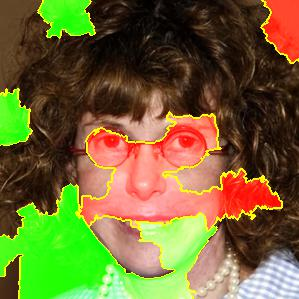
\includegraphics[width=0.3\textwidth]{figures/limeExample.jpg}
  \caption{Example explanation with lime on image from our own data. Red parts show segments contributing to classification as real. Green parts show patches that influence image to be classified as fake.}
  \label{fig:limeexample}
\end{figure}

\section{Databases}

A major problem in comparing detection methods are the different performance metrics and especially the different datasets used for their evaluation. A classifier may be tested on a proprietary database, that may not be available to the public. This makes it very difficult to compare results. Moreover, one usually does not know what to expect when applying the classifier to a novel dataset. We distinguish between two cases. Firstly, using a pretrained model, in which case we are concerned about the generalization ability, and secondly, retraining the model on fresh data. In order to compare different detection methods in those two settings, we have created our own database consisting of four datasets. When looking at building a dataset, we consider the following properties: runtime/computational resources needed, diversity of the generated images, quality and resolution of the images.

\begin{table*}
\centering
\begin{tabular}{c||cccc}
\ &
\textbf{Source Reals} & \textbf{Source Fakes} & \textbf{Generation Method} & \textbf{Resolution} & \textbf{Ref}  \\
\hline
\hline
\textbf{c0} & FF++ & FF++ & Autoencoder & 100-600px \\
\textbf{c23} & FF++ & FF++ & Autoencoder & 100-600px \\
\textbf{HQ} & FlickrHQ & 100k Faces & Style-GAN & 1024px \\
\textbf{X\textnormal{-}Ray} & FlickrHQ, celebAHQ & FlickrHQ, celebAHQ & Image Processing & 1024px
\end{tabular}
\caption{\label{tb:database}
Overview of our own database collection.
}
\end{table*}

\subsection{FaceForensics++}

The first two datasets were created using the FaceForensics++ Deepfake database, which consists of 1000 real and deepfake videos respectively. The deepfake videos in the database were generated using the \emph{faceswap} github implementation \cite{swap}, which is based on an autoencoder. The first 800 videos were used to generate the training and validation set, with an 80/20 split, while the last 200 videos address the test set. One frame was extracted from each video for the test set. As such, it contains 400 images, 200 real and 200 fake. The two datasets only differ in the training set size and compression, with the more compressed dataset being bigger (30k vs 100k images). The compression does not affect the resolution of the videos. We refer to the two datasets as \emph{c0} and \emph{c23}, the number standing for the compression rate factor of the h264 encoded video. Note that the c23 dataset is visually almost identical to the raw, c0 dataset, but takes up 50 times less space.

When looking at the properties, we highlight the following: fast runtime, low diversity and average quality, medium to low resolution. The runtime is mostly due to the face detection required for each extracted frame. This is done using the dlib \cite{dlib09} face detector. By skipping the generation part, we remove the most time-consuming part of the data acquisition process, as a traditional autoencoder approach needs to be trained for fake video separately. We have some diversity by adapting the number of frames extracted from one video, which gives us different head poses. Diversity is limited however by the size of the video database. The resolution of the extracted images depends on two factors. The resolution of the video and the framing of the person in the video, i.e., the relative size of the face in the frame. The images have a resolution between 100x100 and 600x600. We also found that resizing them to a common dimension noticeably degrades the classifier performance. The quality is average because the fake videos in the FF+ dataset were not handpicked, which results in several very unrealistic looking deepfakes.

This pair of datasets allows us to evaluate the effects of compression on the classification performance, in a scenario typically found online. It also addresses videos, as opposed to still images and gives an indication if the methods are suitable for such a setting.

\subsection{HQ Dataset}
Our HQ dataset is composed of 10k real images from FlickrHQ and 10k high quality fake images from 100K Faces \cite{karras2019style}, generated using Style-GAN. These are all high-resolution images with 1024x1024 pixels. We used 8000 pictures for training, 1000 for validation and 1000 for testing. As a complete image dataset, we cannot talk about the runtime required for generation. The diversity of the images is average but cannot be easily extended without incurring a significant time penalty from generation. Although technically not deepfakes, these synthesized images provide a good test for detection methods because of their high-resolution and high-quality and they fall under the same umbrella of manipulation.

\subsection{X-Ray Dataset}
Our last dataset was generated using a computer vision approach described in \cite{li2020face}. The method proceeds in the following way: first, a similar target image is selected. To compute the similarity, the method examines the placement of facial features and computes the Euclidean distance between the facial landmarks of two candidate images. Subsequently, the source face is morphed onto the target picture by warping and blending. This is done by using a mask initialized to the convex hull of the facial landmarks of the source image. An affine transformation is then performed on the mask, which may reduce its size to cover just a part of the original face. This allows, for instance, to only swap the nose of a person. Finally, color correction is performed on the image.

Being computer vision based, the X-Ray method is significantly more lightweight than a traditional autoencoder deepfake approach while still producing high resolution, good quality images. Since it is not a deepfake method, it also lacks the typical artifacts found in these. According to the authors, this should improve the generalization results of classifiers. It is also the most versatile dataset, as it may be easily expanded by generating more images when novel real images are available.
In our attempt to find what helps a classifier be more general, we try to reproduce their findings in our experiments. The absence of low level artifacts, like textures introduced by a deepfake generator, should guide the classifier to more high level features (crop and paste regions).

\section{Detection Methods}
Apart from handcrafted detection methods, most classifiers are based on machine learning. But they vary a lot, ranging from simple logistic regression to neural nets with tens of millions of parameters. We focus on two very different methods, a traditional CNN approach based on the Xception architecture and a method based on the frequency spectrum of an image. The former gives us a baseline for the performance of a state-of-the-art architecture while the latter method explores an promising and less common approach.

\subsection{Xception Net}
The Xception architecture \cite{chollet2017xception} is a state-of-the-art CNN used for many classification problems. We have used the FaceForensics++ implementation with slight modifications. The initialization is done using the weights from the ImageNet trained model and only the last layer is replaced by a fully connected (FC) layer with two outputs, accounting for the real and fake classes. Using an already pre-trained net, two simple approaches exist to extend the model. On the one hand, \emph{Transfer Learning} is used for fine tuning the model, updating all the weights of the network, on the other hand, one can use the existing model as a feature extractor by solely updating the last (classification) layer. We used early stopping and learning rate decay in order to increase performance on difficult datasets.

The Xception Net has a high capacity and that is a main reason why it can adapt to different tasks with very good performance. But once trained on a specific task, we expect low generalization because of overfitting on that particular dataset. We have tried to address this by adding regularization in the form of dropout and weight decay. Another downside is the long training times required in comparison to shallow classifiers.

\subsection{Classifiers trained on the frequency spectrum}
Using the frequency spectrum as input for the classification has one big advantage, namely that the training can be performed using shallow classifiers ,like support vector machines, or neural networks with a small number of layer. To understand the processing pipeline to obtain the input features we refer the reader to the original paper of \cite{durall2020unmasking}. An important aspect that should be kept in mind when training with the frequency spectrum is that accuracy can be significantly increased if we crop and keep only the face area of the image. This will leave out other textures that might appear in the background. Thus, we only used input features that are relevant.

As a shallow classifier, we used an SVM with radial kernel. Usually, the training time is reduced. The only exception are really big datasets with ~100.000 input images, however even in this case it is faster than using the Xception Net. We used an already existing Python implementation from the library \textit{scikit-learn}\cite{scikit-learn}. We also implemented a fully connected neural network with four layers as an alternative classifier and compared accuracy and generalization power.


\section{Experiments}
%In our experiments, we have compared the frequency spectrum to the CNN classifier. We performed tests on all our four datasets and explored generalization by cross-testing {\color{red}(Is there some common term for this)}, training on one dataset and testing on another. We then use LIME to gather more insights into what our models consider to be differentiating features between real and fake images.

The main part of our experiments is to compare our two models and, especially, analyze how they generalize amongst different datasets. The idea is to train a model on a dataset and, subsequently, to test it on all the other datasets. This is repeated for all model-training-data combinations. Finally, to qualitatively understand how the models decide, we use the Lime framework to analyze the decision boundaries.

\subsection{Training}
The CNN classifier was initialized with an ImageNet model and trained for a maximum of 30 epochs, updating all the weights, not just the final fully connected layer. The Adam optimizer was used. We used the validation loss to trigger early stopping for all datasets, which generally resulted in 6 to 7 epochs. The only exception was the X-Ray dataset, which needed around 28 epochs to converge. It is also the only instance where we needed to use learning rate decay to improve performance. With these measures we insured that the training ran until convergence and didn't overfit on the training set.

\begin{table}
\[\begin{array}{c|cccc}
\tikz{\node[below left, inner sep=1pt] (def) {\textbf{Train}};%
      \node[above right,inner sep=1pt] (abc) {\textbf{Test}};%
      \draw (def.north west|-abc.north west) -- (def.south east-|abc.south east);}
 & \textbf{c0} & \textbf{c23} & \textbf{HQ} & \textbf{X\textnormal{-}Ray}\\
\hline
\textbf{c0} & 0.99 & 0.693 & 0.5 & 0.501\\
\textbf{c23} & \textbf{0.99} & 0.987 & 0.5 & 0.501\\
\textbf{HQ} & 0.5 & 0.5 & 0.994 & 0.498\\
\textbf{X\textnormal{-}Ray} & 0.6 & 0.553 & 0.509 & 0.975\\
\end{array}\]
\caption{\label{tb:xception-cross}
Results of training and cross-testing between different datasets for the Xception Net.
}
\end{table}


On the frequency side, the SVM has been trained using the standard library functions. For the Frequency Neural Net (FreqNN), we trained for a maximum of 300 epochs and used early stopping set on 30 epochs. Other changes performed to the architecture did not improve the accuracy since the dimensionality is reduced and the used classifiers have a simple architecture. For the frequency spectrum, the only changes that might influence the accuracy dramatically are those performed while computing the input features and other preprocessing done to the images. 

\subsection{Test and Analysis}
\begin{table*}[!t]
\[\begin{array}{c|cccc}
\tikz{\node[below left, inner sep=1pt] (def) {\textbf{Train}};%
      \node[above right,inner sep=1pt] (abc) {\textbf{Test}};%
      \draw (def.north west|-abc.north west) -- (def.south east-|abc.south east);}
 & \textbf{c0} & \textbf{c23} & \textbf{HQ} & \textbf{X\textnormal{-}Ray}\\
\hline
\textbf{c0} & 0.92 \ | \ 0.90 & 0.64 \ | \ 0.72 & 0.45\ | \ 0.44 & 0.52\ | \ 0.58\\
\textbf{c23} & \textbf{0.88}\ | \ \textbf{0.86} & 0.84\ | \ 0.83 & 0.48\ | \ 0.43 & 0.49\ | \ 0.54\\
\textbf{HQ} & 0.49\ | \ 0.50 & 0.49\ | \ 0.49 & 1.00\ | \ 1.00 & 0.49\ | \ 0.51\\
\textbf{X\textnormal{-}Ray} & 0.49\ | \ 0.56 & 0.49\ | \ 0.56 & 0.44\ | \ \ \ ? \ \ \ & 0.78\ | \ 0.75\\
\end{array}\]
\caption{\label{tb:frequency-cross}
 Accuracy results of training and cross-testing between different datasets for the frequency classifiers (SVM based vs neural network (NN) based). The accuracy values are in the format SVM|NN.
}
\end{table*}
After having trained every model-dataset pair, we performed the cross-testing. The results for the Xception Net can be seen in table \ref{tb:xception-cross}. The results for the frequency analyzers can be seen in table \ref{tb:frequency-cross}. The diagonal entries show the accuracy of a model when the training and test images stem from the same dataset. More interesting for the analysis of generalization, however, are the off-diagonals. These show the cases where the training and test sets do not stem from the same collection.

Our main findings are
\begin{enumerate}
    \item None of the methods or datasets helps in generalizing the detection to unseen data
    \item Repeating the first point, but making it explicit: The X-Ray dataset, contrary to our expectations and the findings of \cite{li2020face}, does not help in terms of generalization
    \item Slightly compressing the training data may help to make the detection more robust
    \item For the frequency spectrum classifier, the neural network did not improve the overall performance of the SVM variant
    \item Frequency analyzers are vulnerable to compression and resizing artifacts
\end{enumerate}

The first point can be seen in the very low off-diagonal values. This again underlines that the task to detect fakes is not trivial. The main issue is that in a real scenario, one does not know how the fake was created (not to mention whether the given image/video is fake at all). We have shown that neither the Xception Net, nor the frequency classifiers are able to generalize to unseen data. Moreover, touching on the second point, we also have shown that none of the datasets, including the X-Ray data, helped with finding common patterns between the generation methods.


Although the X-Ray method promises to find the cropping and pasting regions of the face masks, we were not able to reproduce these results. Possible reasons can be: a) we solely used high resolution images. One may vary more; b) our parameters like compression, and down- and upsampling again were too strong; c) the pristine dataset is not good (too simple, etc.); d) the difficult training process may already point to some issues present in our case that needs to be further investigated.

Furthermore, given our c0 and c23 datasets, we can show that in all our methods (Xception, FreqNet, Frequency+SVM) the slight compression in training helped in generalizing to detecting uncompressed data (see bold values in both tables). Training on the uncompressed data and predicting on the compressed one, on the contrary, did not result in good accuracies.

Finally, we also have shown that the frequency method attained comparably bad results when handling compressed data. The relatively low diagonal values for c23 and X-Ray in table \ref{tb:frequency-cross} show this. Whilst c23 is compressed, X-Ray contains both compressing and other blurring/resizing operations, that possibly distort the image frequencies.

\subsection{Visualization}
\begin{figure}
    \centering
    \begin{subfigure}[b]{0.2\textwidth}
        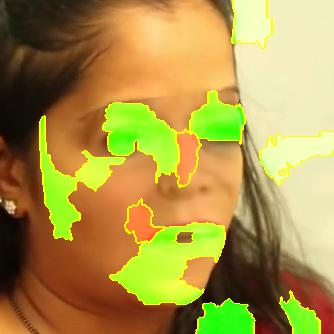
\includegraphics[width=\textwidth]{figures/SVM_c0_fake.jpg}
        \caption{SVM on c0}
        \label{fig:svm-c0}
    \end{subfigure}
    \begin{subfigure}[b]{0.2\textwidth}
        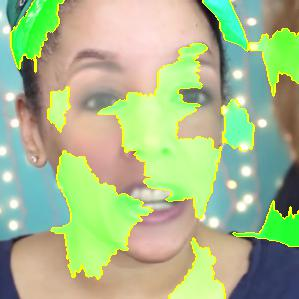
\includegraphics[width=\textwidth]{figures/xception_c23_fake.jpg}
        \caption{Xception on c23}
        \label{fig:xception-c23}
    \end{subfigure}
    
    
    \begin{subfigure}[b]{0.2\textwidth}
        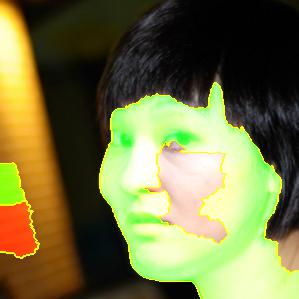
\includegraphics[width=\textwidth]{figures/xception_xray_fake.jpeg}
        \caption{Xception on X-Ray}
        \label{fig:xception-xray}
    \end{subfigure}
    \caption{Explanations using Lime. Green color depicts regions that contribute to classify image as fake (and conversely, red as real). All images were correctly classified as being fakes in each case.}\label{fig:explanations}
\end{figure}
For every model-training-data pair, we further performed explainability analyses with the Lime tool. Whilst there exist detection methods that explicitly use hand-crafted features such as facial landmarks etc., the models we used were either completely black box (Xcpetion Net) or utilized abstract higher level features (frequencies). Our goal was to get an intuition on what visual features our methods focus on in their decisions since those are not modelled explicitly.

Figure \ref{fig:explanations} shows some example outputs of the Lime tool. Each of the images are from different datasets as the image labels show. Moreover, all of the images are fakes and correctly categorized as such. One can see that the SVM on the c0 data mainly focused on the eye and mouth region, which perfectly fits the findings in deepfake detection research \cite{Mirsky2021,nguyen2021deep,Tolosana2020}. It is assumed that most of the generators suffer in these regions. The Xception Net trained on the c23 also focused on similar areas (nose, eyebrows, mouth, etc.), and can be seen in figure \ref{fig:xception-c23}. The Xception trainined on X-Ray, on the contrary, focused on broader face regions as shown in \ref{fig:xception-xray}. We assume that the X-Ray data made the detector learn the face mask areas as it was promised and expected, although not helping in the ability to detect fakes from unknown sources. In order to be able to make stronger assumptions, one should do more experiments with the X-Ray method as described in the Conclusion section.

\subsection{Conclusion}
Deepfake detection is a hard task as argued in many research papers \cite{Mirsky2021,nguyen2021deep,Tolosana2020}. The difficulty stems from the fact that the classifiers  overfit to a given dataset, and thereby solely discern patterns that come with the underlying generation methods.

We were able to reproduce these findings, and have shown that neither the Xception Net, nor the frequency classifiers are able to overcome this issue. We therefore created our own database with publicly available images and the image processing algorithm as used in the X-Ray paper \cite{li2020face}. Although having a promising outlook with the X-Ray dataset, we were able to show that it was not able to provide generalization in our case. Either the method is not suitable in all scenarios, or we had some problems that need still to be analyzed in a future work.

Further future work can be focused on alleviating the issue in generalization by mixing different datasets for training. Although this might improve the performance on known datasets drastically, it still needs to be investigated in how far unseen (novel) methods can be detected with this approach. One could focus on creating a dataset that includes as many different generation methods as possible (CNN-based, GAN-based, VAE-based, etc.) and to speculate that future generators share common features with at least one of the methods involved.

Other partial solutions would involve methods such as few-shot/one-shot learning as described in \cite{Aneja2020,Cozzolino2018}. This approach would help if one has access to only a few fakes that can already be defined as such, making the model trainable with as few samples as possible.

Finally, having analyzed a large amount of scientific publications and projects, we think that the most promising approach would be to pose the task as an anomaly detection task as in \cite{anomalyPaper}. The idea is to use all existing data that one has (including real and fakes from different sources) and to learn common structures amongst them. When a new image needs to be categorized, the model will use this knowledge to perceive in how far a new image deviates from the real ones, and will output a class accordingly.



% Includes only your custom bibliography per default. See above for how to include anthology files.
\bibliography{custom}
\bibliographystyle{acl_natbib}


\end{document}
